\documentclass[12pt]{article}
\usepackage{amsmath, amssymb,amsthm,multicol,graphicx,tikz}
%\usepackage[backend=biber,style=ieee,sorting=none,sortcites=true]{biblatex}
\usepackage[ruled,vlined]{algorithm2e}
\usepackage{makeidx}
\usepackage{float}
\usepackage{xcolor}
\usepackage{forest}
%\usepackage[colorlinks=true,citecolor=blue]{hyperref}
\usepackage{hyperref}
\textheight22cm
\textwidth17cm
\oddsidemargin0cm
\evensidemargin0cm
\setlength{\topmargin}{-0.2in}
\newcommand{\ds}{\displaystyle} %use before summations or integrals
\newcommand{\ZZ}{\mathbb{Z}}%shorthand for integers
\newcommand{\QQ}{\mathbb{Q}}%shorthand for rational numbers
\newcommand{\RR}{\mathbb{R}} %shorthand for real numbers
\newcommand{\CC}{\mathbb{C}} %shorthand for complex numbers
\newcommand{\sym}{\mathcal S}

\newtheorem{prop}{Proposition}   %Use this to start a numbered Proposition
\newtheorem{lem}{Lemma} %Use this to start a numbered Lemma
\newtheorem{thm}{Theorem} %Use this to start a numbered Theorem
\newtheorem{defn}{Definition} %Use this to start a numbered Definition
\newtheorem{ex}{Example} %Use this to start a numbered Example
\newtheorem{exc}{Exercise} %Use this to start a numbered Exercise
%\newtheorem{ex}[thm]{Example}

%\addbibresource{bibliography.bib}

\title{Permutation Pattern Avoidance}
\author{Daniel Evans, Grace Hansen, \\Andrew Mortensen, Tran Khanh Tra (Fay) Nguyen}
\date{May 2026}

\makeindex
\begin{document}

\maketitle
\section{Introduction}
% Motivate by mentioning take-home ordering problem
Pattern avoidance is an extremely active area of enumerative combinatorics. The central questions in this research are \textit{which permutations avoid certain patterns?}, \textit{how many are there?}, and \textit{what are some interesting properties/applications of this type of permutations?} First, we will take a look at methods of counting the number of permutations that avoid patterns of different lengths, taking us all the way to the cutting edge of research in the area. Next, we will explore a generalized version of pattern avoidance and other properties and visualizations of pattern-avoiding permutations. Finally, we will view the topic from a computer science perspective, focusing on its applications in stack sorting.

%Informally, a permutation of the elements in $[n]=\{1,2,\dots,n\}$ that avoids 



\section{Pattern-avoiding Permutation}

Given a set of integers $\{1,2,\ldots,n\}$ ($n \in \mathbb{N}^*$) denoted by $[n]$, we define the symmetric group on this set as $\mathcal{S}_n$, the group of all possible permutations of the set $[n]$. We already learned in class that the cardinality of this group is $n!$, or $|\mathcal{S}_n| = n!$.

Let $\pi \in \mathcal{S}_n$ be a permutation of $[n]$, then we can write $\pi$ as an one-line notation:

$$\pi = \pi_1\pi_2\pi_3\ldots\pi_n$$

Before we continue with permutations, we need to review an important math concept: \textbf{relative order}\index{relative order}. This is the specific, fixed sequence in which a subset of elements in a permutation appears in relation to each other, regardless of the elements between them or the overall arrangement.


We then choose a positive integer $m$ such that $m \leq n$. We have $\mathcal{S}_m$ to be the set of all possible permutations of the set $[m]$. Let $\sigma \in \mathcal{S}_m$ and $\sigma =\sigma_1, \sigma_2, \sigma_3, \ldots, \sigma_m$. If there exist indices $1\leq i_1 < i_2 < i_3 < \ldots < i_m\leq n$ such that $\pi_{i_1}, \pi_{i_2}, \pi_{i_3}, \ldots, \pi_{i_m}$ have the same relative order as $\sigma_1, \sigma_2, \sigma_3, \ldots, \sigma_m$, we can conclude that $\pi$ contains $\sigma$ with $\pi_{i_1}, \pi_{i_2}, \pi_{i_3}, \ldots, \pi_{i_m}$ as the occurrence \index{occurrence} of $\sigma$ in $\pi$, and $\sigma$ is a pattern\index{pattern}.

We can now define the most important concept of this paper:
\begin{defn}
Given a permutation $\pi \in \mathcal{S}_n$, if $\pi$ does not contain the pattern $\sigma$, $\pi$ avoids $\sigma$ or $\pi$ is a \textbf{$\sigma$-avoiding permutation}\index{$\sigma$-avoiding permutation}.\cite{elizalde2004}
\end{defn}

\begin{ex}
    We have the permutation $\pi_1 = 653421, \pi_2=654321$, and $\sigma = 231$. Then we have $\pi_1$ contains $\sigma$, because we have the subsequence $\pi_3\pi_4\pi_6=341$ has the same relative order as $231$. Meanwhile, $\pi_2$ does not contain the pattern $\sigma$, or $\pi_2$ is $231-$avoiding.   
\end{ex}

\begin{defn}
For a pattern $\sigma$, let $\mathcal{S}_n(\sigma)$ denote the set of permutations that belong to $[n]$ that avoid $\sigma$. Then $s_n(\sigma):=|\mathcal{S}_n(\sigma)|$ counts the number of $\sigma$-avoiding permutations of size $n$. 
\end{defn}
%Should we move this down to the property section?
%double check 
\begin{defn}
    Let $\sigma$ and $\tau$ be permutations of equal length. If $s_n(\sigma)=s_n(\tau)$ for all $n \in \mathbb{N}^*$, then $\sigma$ and $\tau$ are called \textbf{Wilf equivalent}\index{Wilf equivalent}.
\end{defn}
% All permutations of size 3 are Wilf equivalent (proof?)

There are three \textbf{symmetries} of permutations that preserve Wilf equivalence. A permutation $\pi =\pi_1\;\pi_2\dots \pi_n$ is Wilf equivalent to:
\begin{enumerate}
    \item its \textbf{reverse} $\pi^r=\pi_n\;\pi_{n-1}\dots \pi_1$,
% Should this be a definition/theorem/lemma?
% Commas or not?
    \item its \textbf{complement} $\pi^c=(n+1-\pi_1)\;(n+1-\pi_2)\dots(n+1-\pi_k)$,
    \item its \textbf{inverse} $\pi^{-1}$ in the symmetric group, i.e. the permutation that undoes $\pi$. % Elaborate?
\end{enumerate}
Notice that Wilf equivalence is an equivalence relation and so it partitions $\sym_n$ into equivalence classes.
% Equivalence relation explain

\section{Classical Pattern-Avoiding Permutations}

A natural question arises from pattern avoidance: how many permutations avoid a specific pattern? Specifically, how many permutations of a certain length avoid a pattern in a certain Wilf equivalence class. We will see how finding the closed formula for the sequence $s_n(\sigma)$ starts out simple with short patterns $\sigma$ before quickly growing in complexity when the pattern size increases. This will demonstrate how the longer a pattern is, the less restrictive it is on patterns avoiding it, which makes them more difficult to count.

% \sym_0?
\subsection{Classical Patterns of Length $1$}
There is only one permutation in the symmetric group on $[1]$: $\sym_1=\{1\}$. The only way to avoid the pattern $\sigma=1$ is by having an empty permutation. Therefore, we have $$s_n(1)=\begin{cases} 
  1 & \text{if } n=0 \\
  0   & \text{if } n\neq0 
\end{cases}\;\;.$$

\subsection{Classical Patterns of Length $2$}
There are two permutations of $[2]$: $S_2=\{12,21\}$. Since these patterns are reverses of each other, they are Wilf equivalent. Thus, we will only need to calculate $s_n$ for one of them, 12. The permutations that avoid 12 are those whose elements are strictly decreasing. For any $n$ the only strictly decreasing permutation of $[n]$ is $n\;(n-1)\cdots2\;1$. Therefore, $s_n(12)=1$ for all $n\geq0$.
% Should it be >0? Should we even consider the empty permtation? If so, mention somewhere that it avoids every nonempty pattern and mention s_0(p) if that's a thing.
By Wilf equivalence, $$s_n(\sigma)=1\;\;\text{for all}\;\;\sigma\in\sym_2\;\;\text{and}\;\;n\geq0.$$

\subsection{Classical Patterns of Length $3$}

There are six permutations of $[3]$: $\sym_3=\{123,132,213,231,312,321\}$. By symmetries, we know that $\{123,321\}$ and $\{132,213,231,312\}$ are sets of Wilf equivalent permutations. Therefore, either these are our Wilf equivalence classes or all of $\sym_3$ is Wilf equivalent. Thus, it will suffice to count pattern-avoiding permutations $s_n$ for one pattern in each class.

Next, we will take a look at two bijection proofs in order to count

\subsubsection{321-avoiding permutations}
\begin{thm}
    The number of 321 avoiding permutations of length $n$ is the same as the number of Catalan paths from $(0,0)$ to $(n,n)$ for $n\geq0$, or $$s_n(321)=c_n.$$
\end{thm}
\begin{proof}
    Let $C_n$ denote the set of Catalan paths from $(0,0)$ to $(n,n)$. Using the bijection discovered by Rotem in 1975\cite{rotem_correspondence_1975}, we will prove that $s_n(321)=c_n$.

    In a permutation $\pi_1\,\pi_2\dots\pi_n$, we call $\pi_i$ a \textbf{left to right maximum} if it is larger than anything to its left, or $\pi_j<\pi_i$ for all $j<i$. Let $M_\pi$ denote the set of left-to-right maxima and let $N_\pi$ denote the other elements of $\pi$. Notice that $\pi$ avoids the pattern 321 if and only if the elements of $N_\pi$ appear in increasing order in $\pi$. This is because if there is decrease $\pi_j>\pi_k$ ($j<k$) and $\pi_j,\pi_k$, aren't left-to-right maxima, then there is another element $\pi_i$ such that $\pi_i>\pi_j>\pi_k$ and $i<j<k$, giving us a 321 pattern. To prove the other direction, we assume that there are elements $\pi_i>\pi_j>\pi_k$ such that $i<j<k$. Then $\pi_j,\pi_k\in N_\pi$, giving us a decrease in $n_\pi$. 
    
    Using this concept, we can assign a \textit{ballot-sequence} to each permutation in $S_n(321)$. A \textbf{ballot-sequence} $b_1\,b_2\dots b_n$ of nonnegative integers have two conditions:\begin{enumerate}
        \item $b_1\leq b_2\leq\dots\leq b_n$ and
        \item $0\leq b_i\leq i-1$ for each $i=1,2,\dots, n$.
    \end{enumerate}
    Now, each permutation $\pi=\pi_1\,\pi_2\dots\pi_n$ in $S_n(321)$, we can construct a ballot-sequence $b=b_1\,b_2\dots b_n$ of length $n$ with the following rules: \begin{enumerate}
        \item $b_1=0$;
        \item $b_{i}=b_{i-1}$ if $\pi_i$ is a left-to-right maximum;
        \item $b_i=\pi_i$ otherwise.
    \end{enumerate}

    \begin{ex}\label{PermToBallot}
        Consider the permutation $\pi=14235\in S_5(321)$. To turn this into a ballot-sequence, we start with $b_1=0$. Now, since $\pi_2=4$ is a left-to-right maximum, we have $b_2=b_1=0$. Next, $\pi_3=2$ and $\pi_4=3$ are not left-to-right maxima, so $b_3=\pi_3=2$ and $b_4=\pi_4=3$. Finally, $\pi_5=5$ is a left-to-right maximum, so $b_5=b_4=3$. So, our final sequence is $b=00233$, which is a valid ballot-sequence.
    \end{ex}
    
        
    Notice that under this construction, each $b_i$ can either be 0 or an element of $[n]$. Furthermore, the element of $\pi$ equal to $n$ is always a left-to-right maximum, so $0\leq b_i\leq n-1$ for all $i=1,2,\dots,n$.
    
    Now, we will prove that that this construction always yields a valid ballot-sequence by checking that both conditions are satisfied.
    \begin{enumerate}
        \item Suppose the permutation $\pi\in S_n(321)$ corresponds to a ballot-sequence $b$ such that $b_j>b_{j+1}$ for some $j=1,2,\dots,n-1$. If $b_j=0$, we have $0>b_{j+1}$ which contradicts the fact that each $b_i<0$. Now, suppose $b_j\in[n]$. By the rules of our construction, $b_j$ must be equal to some $\pi_k\in N_\pi$ such that $k\leq j$. Hence, $\pi_k>\pi_{j+1}$ for some $k<j+1$. Since $a_{j+1}\in N_\pi$, we have a decrease in $N_\pi$. This implies there is a 321 pattern in $\pi$ which contradicts our assumption that $\pi\in S_n(321)$. Therefore, $b_j\leq b_{j+1}$ for all $j=0,1,\dots n-1$, satisfying the first condition.

        \item Suppose the permutation $\pi\in S_n(321)$ corresponds to a ballot-sequence $b$ such that $b_j>j-1$ for some $j=1,2,\dots,n-1$. Since $j\geq1$, we know $b_j>j-1\geq0$. Since $b_j$ is nonzero, $b_j=\pi_k$ for some $\pi_k\in N_\pi$ such that $k\leq j$. Therefore, $\pi_k>j-1\geq k-1$. 
        
        Since $b_j>0$, there is at least one element to the left of $\pi_k$. There also must be at least one element to its right of $b_j$ because if $j=n$, then $b_n>n-1$ which contradicts the fact that each $b_i\leq n-1$.
        
        Now, since $\pi_k$ is not a left-to-right maximum, there must be some element to its left that is greater than it. Thus, since there are $k-1$ elements to the left of $\pi_k$, at most $k-2$ of them are less than $\pi_k$. But since $\pi_k>k-1$, there are at least $k-1$ elements in $\pi$ that are less than $\pi_k$. By the Pigeonhole Principle, at least one element less than $\pi_k$ must be to its right. Therefore, $\pi_k$ has a greater element somewhere to its left a lesser element somewhere to its right, which is a 321 pattern in $\pi$. This contradicts our assumption that $\pi\in S_n(321)$ and so $b_i\leq i-1$ for all $i=1,2,\dots n$. Since we also know that each $b_i\geq0$, satisfying condition 2.
    \end{enumerate}
    Using ballot-sequences, we can define a function $f:S_n(321)\rightarrow C_n$. For any $\pi\in S_3(321)$, we can construct a ballot sequence $b=b_1\,b_2\dots b_n$. From this ballot sequence we can construct a lattice path from $(0,0)$ to $(n,n)$ by letting each $b_i$ correspond to a rightward move from $(i-1,b_i)$ to $(i,b_i)$ and filling in upward moves whenever $b_i<b_{i+1}$. 
    \begin{ex}\label{BallotToPath}
        The lattice path corresponding to the ballot-sequence in Example \ref{PermToBallot}, \textcolor{blue}{00}\textcolor{red}{2}\textcolor{green}{33}, is \textcolor{blue}{RR}UU\textcolor{red}{R}U\textcolor{green}{RR}UU:\\
    
    
    \begin{center}
    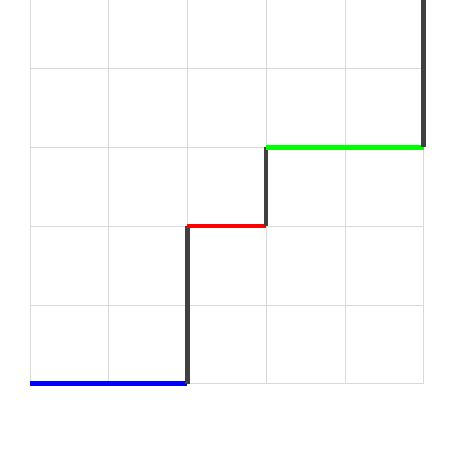
\begin{tikzpicture}
    \draw[help lines, color=gray!30] (0,0) grid (5,5);
    
    \draw[ultra thick, blue] (0,0) -| (2,0);
    \draw[ultra thick, darkgray] (2,0) -| (2,2);
    \draw[ultra thick, red] (2,2) -| (3,2);
    \draw[ultra thick, darkgray] (3,2) -| (3,3);
    \draw[ultra thick, green] (3,3) -| (5,3);
    \draw[ultra thick, darkgray] (5,3) -| (5,5);
    \end{tikzpicture}
    \end{center}
    \end{ex}
    \vspace{1cm}
    For any $\pi\in S_n(321)$, let $f(\pi)$ be the lattice path formed by the ballot-sequence constructed from $\pi$. So in our from our examples, we have $f(14235)=RRUURURRUU$. Since a ballot-sequence of length $n$ always results in a path with $n$ rightward moves at increasing $y$ values and $n$ moves upward that connecting them, a ballot path always yields a lattice path from $(0,0)$ to $(n,n)$. Furthermore, since each $b_i\leq i-1$, the $y$ value of the path can never exceed the $x$ value. Therefore, each $f(\pi)$ is a Catalan path from $(0,0)$ to $(n,n)$. Now, since our first construction yields a single, definitive ballot-sequence for each permutation and our second construction assigns exactly one Catalan path to each ballot sequence, $f$ is well defined.

    To show that this is a bijection, we can prove that $f$ has a well defined inverse, $f^{-1}$. First, we can turn a Catalan path in $C_n$ into a ballot-sequence of length $n$ by listing each rightward moves from left to right by it's $y$ value. This is precisely the reversal of the Catalan construction process and it can be done to any Catalan path to obtain a ballot sequence. Since the $y$ value of the first rightward move is 0 and the subsequent rightward moves are increasing in $y$ value, $0\leq b_1\leq b_2\leq\dots\leq b_n$ in the resulting ballot sequence. Also, since the $y$ value of the $i$th rightward move cannot be more than $i-1$, we have $b_i\leq i-1$ for each $i=1,2,\dots n$ in the sequence that results from the reverse construction. Therefore, our reverse construction yields a single ballot-sequence.

    Next, we can reverse our ballot-sequence construction. For any ballot sequence $b=b_1\,b_2\dots b_n$, consider the permutation $\pi$ of $[n]$ constructed using the following instructions. First, for each $b_i\neq b_{i-1}$ for $i=2,3,\dots,n$, let $\pi_i=b_i$. Now fill in the remaining elements of the permutation with the remaining unused elements of $[n]$ in ascending order from left to right.
    % For example
    This is the exact reverse steps of of the ballot-sequence construction because $b_1$ and each repeated become left-to-right maxima in $\pi$ while the rest become elements of $N_\pi$. Since each non-repeated element of $b$ is a unique element of $\{1,2,\dots,n-1\}$, this reverse construction yields a single permutation of $[n]$ for each ballot sequence of length $n$. Since the non-repeated elements appear in ascending order and become the elements of $N_\pi$, we have that the elements of $N_\pi$ appear in ascending order in $\pi$, which implies $\pi\in S_n(321)$.

    Now, define $f^{-1}:C_n\rightarrow S_n(321)$ as the reverse of the second construction ($C_n$ to ballot-sequence) followed by the reverse of the first construction (ballot-sequence to 321 avoiding permutation).

    \begin{ex}
        Using the path from Example \ref{BallotToPath}, we can find $f^{-1}(RRUURURRUU)$.\\
        
        First, using the reverse of the second construction, we have 2 rightward moves at $y=0$, 1 at $y=2$, and 2 at $y=3$. Therefore, the resulting ballot-sequence is $b=00233$.

        Now, using the reverse of the first construction, we will find a permutation $\pi$ from our ballot sequence. The non-repeated elements of our sequence (besides $b_1$) are $b_3=2$ and $b_4=3$. Thus, we let $\pi_3=b_3=2$ and $\pi_4=b_4=3$. Now we have a 3 remaining spots to fill in: $\pi=\_\,\_\,2\,3\,\_$. The unused elements of $[5]$ are 1, 4, and 5, so we put them in the empty spaces in ascending order to obtain $\pi=14235$. Therefore, we have $$f^{-1}(RRUURURRUU)=14235.$$
        Recall that $f(14235)=RRUURURRUU$, so $f^{-1}(f(14235))=14235$.
    \end{ex}

    
    We showed that each reverse construction yields one definitive result for each input, which implies $f^{-1}$ is a well defined function. Now, since each construction is the reverse of its respective base constructions, we have that $f^{-1}(f(\pi))=\pi$ for any $\pi\in S_n(321)$, proving that $f^{-1}$ is the true inverse to $f$.
    % See running example, that should show that we ended up where we started
    Since $f$ has a well defined inverse, it is a bijection. Therefore, $|S_n(321)|=|C_n|$, or $$s_n(321)=c_n.$$
    
    
    %In the permutation $\pi\in S_n(321)$, the $\pi_k=n$ element splits the permutation into a left and a right part. Since $n$ is the largest element of the permutation, the right side must be strictly increasing. If we saw any decrease, we would have a $321$ pattern beginning with $n$. Therefore, none of the elements on the right are left-to-right maximums and $b_i=\pi_i$ for all $i>k$. Let $\pi_r$ be the largest element to the right of $n$. On the left, we must have no 321 patterns and the subsequence of $\pi_j$ such that $j<k$ and $\pi_j>\pi_r$ must be strictly increasing to avoid a 321 pattern of two elements on the left and one on the right. Therefore, each $\pi_j$ is a left to right maximum
    

    % Why is this a unique ballot sequence?
    % Why is do these correspond to unique Catalan paths?
    % Well-defined?
    % Inverse
\end{proof}

Since $123$ is the reverse of $321$, we also know that $s_n(123)=c_n$ by Wilf equivalence.

Now, let's look at a bijection that counts patterns that avoid 123 and patterns that avoid 132.

\subsubsection{$132$-avoiding permutations}

In this subsection, we introduce you to a new definition: \textbf{Dyck path}\index{Dyck path}. This is a lattice path in the plane $\mathbb{Z}^2$ consisting of UP (diagonally) steps $(1,1)$ and DOWN (diagonally) steps  $(1,-1)$ which goes from $(0,0)$ to $(2n,0)$ and never goes below the $x$-axis (the $x-$coordinate will never be smaller than $0$). Let $\mathcal{D}_n$ be the set of Dyck paths from $(0,0)$ to $(2n,0)$. According to the publication published by Luo and Zhou in 2025 \cite{Luo2025}, the number of Dyck paths of length from $(0,0)$ to $(2n,0)$ is exactly equal to the $n^{th}$ Catalan number ($C_n$).

We can define a function $\Phi: \mathcal{S}_n(132) \rightarrow \mathcal{D}_n$ that maps a $132-$avoiding permutation $\pi =\pi_1\pi_2\pi_3\ldots \pi_n$ to a corresponding Dyck path from $(0,0)$ to $(2n,0)$. With each $\pi_i$ ($1 \leq i \leq n$), we follow these steps to create the corresponding Dyck path \cite{Krattenthaler2000}: 

\begin{enumerate}
    \item We define $h_i$, the number of elements in $\pi_{i+1}\pi_{i+2}\ldots \pi_{n}$ that are larger than $\pi_i$
    \item We go UP for a sufficient number of steps (or we can stay at the same position) such that we arrive at the point $(x,y)$ that has $y=h_i + 1$ 
    \item We go DOWN for one step from $(x,y)$ to $(x + 1,y - 1)$
\end{enumerate}

For example, we have $\pi = \textcolor{blue}{5}\;\textcolor{red}{3}\;\textcolor{purple}{2}\;\textcolor{green}{4}\;\textcolor{orange}{1}$ which is $132-$avoiding. The first element is $\pi_1=5$, and there is no element in $3\;2\;4\;1$ which is larger than $5$. Therefore, we have $h_1=0$, so the path starts with one UP step followed by a DOWN step (color \textcolor{blue}{blue}). The second element is $\pi_2=3$, and there is $1$ element in $2\;4\;1$ which is larger than $3$. Therefore, $h_2=1$, so the path then goes two UP steps followed by a DOWN step (color \textcolor{red}{red}), etc. The last element is $\pi_5=1$, and there is no larger element after this. Therefore, we have $h_5=0$, and no UP steps need to be taken. We only need to go one step DOWN to reach the $x-$axis. The complete Dyck path $\Phi( \textcolor{blue}{5}\;\textcolor{red}{3}\;\textcolor{purple}{2}\;\textcolor{green}{4}\;\textcolor{orange}{1})$ is show in the figure below:
$$
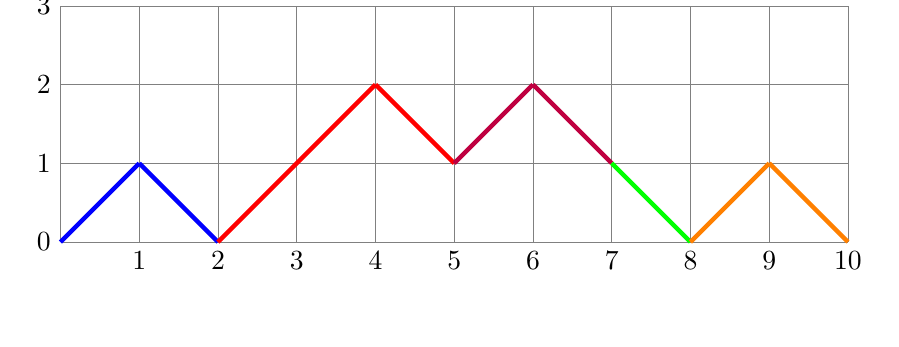
\begin{tikzpicture}[scale=1][H]
    % Draw the grid and diagonal
    \draw[help lines] (0,0) grid (10,3);

    \node[left] at (0,0) {0};
    \node[left] at (0,1) {1};
    \node[left] at (0,2) {2};
    \node[left] at (0,3) {3};
    \node[below] at (1,0) {1};
    \node[below] at (2,0) {2};
    \node[below] at (3,0) {3};
    \node[below] at (4,0) {4};
    \node[below] at (5,0) {5};
    \node[below] at (6,0) {6};
    \node[below] at (7,0) {7};
    \node[below] at (8,0) {8};
    \node[below] at (9,0) {9};
    \node[below] at (10,0) {10};
    \draw[ultra thick, blue] (0,0) -- (1,1);
    \draw[ultra thick, blue] (1,1) -- (2,0);
    \draw[ultra thick, red] (2,0) -- (4,2);
    \draw[ultra thick, red] (4,2) -- (5,1);
    \draw[ultra thick, purple] (5,1) -- (6,2);
    \draw[ultra thick, purple] (6,2) -- (7,1);
    \draw[ultra thick,  green] (7,1) -- (8,0);
    \draw[ultra thick,  orange] (8,0) -- (9,1);
    \draw[ultra thick, orange] (9,1) -- (10,0);
\end{tikzpicture}
$$

We now need to prove that $\Phi$ is bijective. 

\begin{proof}
Let $\pi \in \mathcal{S}_n(132)$, and $\pi = L\;n\;R$ ($n$ at position $1 \leq k \leq n$) with 
\begin{itemize}
    \item $L = \pi_1\pi_2\ldots\pi_{k-1}$
    \item $R = \pi_{k+1}\pi_{k+2}\ldots\pi_{n}$
\end{itemize}

 If there exist $\pi_i \in L$ and $\pi_j \in R$ such that $\pi_i < \pi_j < n$, it creates a subsequence $\pi_i \;n \;\pi_j$, which is an occurrence of $132$. Therefore, every element $\pi_i \in L$ has to be larger than every element $\pi_j \in R$.

 Therefore, we can conclude that:

 \begin{itemize}
    \item $L$ is a permutation of $(k+1)\;(k+2)\ldots n$
    \item $R$ is a permutation of $1\;2\ldots k-1$
\end{itemize}

Besides, $L$ and $R$ have to be $132-$avoiding.

Let $\mathcal{D}_n$ be the set of all Dyck paths going from $(0,0)$ to $(2n,0)$. Every non-empty Dyck path $D \in \mathcal{D}_n$ has at least one time returning to the $x-$axis after. Besides, since the path should never go below the $x-$axis, $D$ will always start with an UP step. Therefore, we can split $D$ into $D = UP\;D_1\;DOWN\;D_2$ with

\begin{itemize}
    \item $UP$: the first UP step of the path
    \item $D_1$: the part of $D$ that stays strictly above the $x-$axis before the first return
    \item $DOWN$: the first DOWN step that touches the $x-$axis for the first time after it begins from $(0,0)$
    \item $D_2$: the remaining part of $D$
\end{itemize}

We define $\Phi$ above as the function that maps $\pi$ to a corresponding $D \in \mathcal{D}_n$. 

If $\pi=\emptyset$, $\Phi(\emptyset)$ will be an empty path. 

For a permutation $\pi = L \; n \; R$, $L$ and $R$ are also $132-$avoiding. And when we reach $\pi_i=n$, there is no more number on its right that is larger than $n$ ($h_i=0$), so the Dyck path has to go from $(x,1)$ to $(x+1,0)$. For every $1 \leq j < i$, $h_j \geq 1$ since $n$ is the largest in the whole permutation. Therefore, when the map reaches $n$, it is the first time that the Dyck path touches the $x-$axis after the beginning. Therefore, this step corresponds to $DOWN$ part in $D$. 
$$ \Phi(\pi) = UP \;\Phi(L) \;DOWN \ \Phi(R)$$

Since $L$ and $R$ are $132$-avoiding, this function is well-defined.

Let $\alpha(L)$ be the permutation obtained by replacing the smallest element by $1$, the second smallest by $2$, and so on. Then $\alpha(L) \in \mathcal{S}_{k-1}(132)$. We also have $R \in \mathcal{S}_{n-k}(132)$.

Therefore, we have:

$$\Phi(\pi)=UP\;\Phi(\alpha(L))\;DOWN\;\Phi(R)$$

We now show that $\Phi$ is a bijection.

We already have $\Phi$ well-defined. 

If $\pi=\emptyset$, then $\Phi(\pi)$ is the empty Dyck path.

If $\pi\neq \emptyset$, then $\pi=L\,n\,R$, and $\alpha(L) \in \mathcal{S}_{k-1}(132)$. We also have $R \in \mathcal{S}_{n-k}(132)$.

We have $\Phi(\alpha(L))$ and $\Phi(R)$ are Dyck paths. Therefore, $UP\;\Phi(\alpha(L))\;DOWN$
is a Dyck path that returns to the $x-$axis for the first time after we start the path, and then $\Phi(R)$ continues as another Dyck path. Hence, $\Phi(\pi)\in \mathcal{D}_n$.

Next, we construct the inverse function $\Gamma$. Let $D\in\mathcal{D}_n$. If $D$ is empty, we define $\Gamma(D)=\emptyset$. Otherwise, $D$ has a unique decomposition $D=UP\;D_1\;DOWN\;D_2$, where $D_1\in\mathcal{D}_a$, $D_2\in\mathcal{D}_b$, and $a+b=n-1$.

Let $\sigma=\Gamma(D_1)\in \mathcal{S}_a(132)$, $\tau=\Gamma(D_2)\in \mathcal{S}_b(132)$.

We define $\Gamma(D) = (\sigma_1+b)(\sigma_2+b)\cdots(\sigma_a+b)\; n\; \tau_1\tau_2\cdots\tau_b.$

Therefore, every element on the left of $n$ is larger than every element on the right of $n$.

We claim that $\Gamma(D)$ avoids $132$. Any $132-$occurrence entirely inside the left part or entirely inside the right part does not exist. A $132-$pattern including $n$ would have to be $x\;n\;y$ where $x < y$. But every element $x$ on the left side of $n$ is larger than every element $y$ on the right of side of $n$, so there exist no $x$ and $y$ such that $x<y$ is impossible. 

Finally, a $132-$pattern using
elements from both sides but not using $n$ is also impossible, because all elements on the
left are larger than all elements on the right. Therefore, $\Gamma(D)\in \mathcal{S}_n(132).$

We also need to prove that $\Phi$ and $\Gamma$ are inverse to each other. With $\pi=L\,n\,R$, $\Phi(\pi)=UP\;\Phi(\alpha(L))\;DOWN\;\Phi(R).$

Applying $\Gamma$ to this path reconstructs the same left part, shifts its values back to
the correct set $L$, inserts $n$, and then reconstructs $R$. Therefore, $\Phi(\pi))=\pi$.

Starting with a Dyck path $D=UP\;D_1\;DOWN\;D_2$, the map $\Gamma$ constructs the corresponding permutation, and applying $\Phi$ recovers
the same decomposition. Therefore, $\Phi(\Gamma(D))=D$.

In conclusion, $\Phi$ is a bijection between $mathcal{S}_n(132)$ and $mathcal{D}_n$. 
\end{proof}

Therefore, we have $\Phi$ as a bijection between $132-$avoiding permutations of $[n]$ and Dyck paths from $(0,0)$ to $(2n,0)$. This implies that the number of $132-$avoiding permutations of $[n]$ is equal to the number of Dyck paths that go from $(0,0)$ to $(2n,0)$, or $s_n(132)=c_n$.

Since $132$, $213$, $231$, and $213$ are Wilf equivalent by symmetries, we know that $s_n(213)=s_n(231)=s_n(312)=s_n(132)=c_n$. 

We also get that $s_n(123)= s_n(321) = c_n$ (from section $3.3.2$). This brings us to an important proposition.

\begin{prop}
    All of the patterns of length $3$ are Wilf equivalent, and $s_n(\sigma)$ with $\sigma$ of length $3$ is always equal to $C_n$.
\end{prop}

\subsubsection{Bonus: $123$-avoiding permutations with Dyck paths}
We can also define a function $\Psi: \mathcal{S}_n(123) \rightarrow \mathcal{D}_n$ that maps a $123-$avoiding permutation of $[n]$ to a Dyck path from $(0,0)$ to $(2n,0)$.

Let $\pi = \pi_1\pi_2\pi_3\ldots\pi_n$ be a $123-$avoiding permutations. For every $\pi_{n-i+1}$ ($1 \leq i \leq n$), we define $m_i = \pi_i$ a \textbf{right-to-left maximum}\index{right-to-left maximum} if it is larger than anything to its right or $m_i = m_{i-1}$ otherwise. Let the base case $m_0=0$. We have $m_j < m_i$ for all $j<i$.
Let $M_\pi$ denote the set of right-to-left maxima, and $s = |M_\pi|$. Besides, we denote the consecutive subsequence of $\pi$ between $m_{i+1}$ and $m_i$ as $w_i$. Therefore, we have:
\begin{align}
\pi = w_sm_sw_{s-1}m_{s-1}\ldots w_1m_1
\end{align}

 Notice that $\pi$ avoids the pattern $123$ if and only if every element in $w_i$ must appear in decreasing order. This is because if there is an increase $\pi_j<\pi_k$ ($j<k$) and $\pi_j,\pi_k \in w_i$, aren't right-to-left maxima, then $\pi_j<\pi_k<m_i$, giving us a $123$ pattern. Besides, all elements in $w_i$ must be smaller than all the elements of $w_{i+1}$.

 So, how can we map this type of permutation to a Dyck path? Now we will read this permutation from right to left using the decomposition (1). With each $m_i$ and $w_i$ ($i$ decrements from $1 \leq i \leq |M_\pi|$), we follow these steps to create a Dyck path\cite{Krattenthaler2000}:

 \begin{enumerate}
     \item We take $m_i - m_{i+1}$ UP steps.
     \item For every consecutive subsequence $w_i$, we take $|w_i| + 1$ DOWN steps ($|w_i|$ is the number of elements of $w_i$).
 \end{enumerate}

Finally, we reflect the newly generated Dyck path over the vertical line. The resulting Dyck path is $\Psi(\pi)$.

 For example, we have $\pi = 5\;8\;3\;2\;7\;6\;4\;1$ which is $123-$avoiding. 

 Going from right to left, we get the table below:
 
$$
\begin{tabular}{|c|c|c|c|}
\hline
$i$ & $m_i$ & $w_i$ & $|w_i|+1$ \\ \hline
$0$& $0$ &  &\\ \hline
$\textcolor{blue}{1}$& $1$ & $\emptyset$ & $1$\\ \hline
$\textcolor{red}{2}$& $4$ & $\emptyset$ & $1$ \\ \hline
$\textcolor{purple}{3}$& $6$ & $\emptyset$ & $1$\\ \hline
$\textcolor{green}{4}$& $7$ & \{$2,3$\} & $3$\\ \hline
$\textcolor{magenta}{5}$& $8$ & \{$5$\} & $2$ \\ \hline
\end{tabular}
$$

With these values, we can draw a Dyck path following the first two steps mentioned above. For example, with $m_1=1$, we can go one UP step from $(0,0)$ to $(1,1)$ (since $m_1 - m_0 =1$) and then take one DOWN step from $(1,1)$ to $(2,0)$ (since $|w_1|+1=1$).

$$
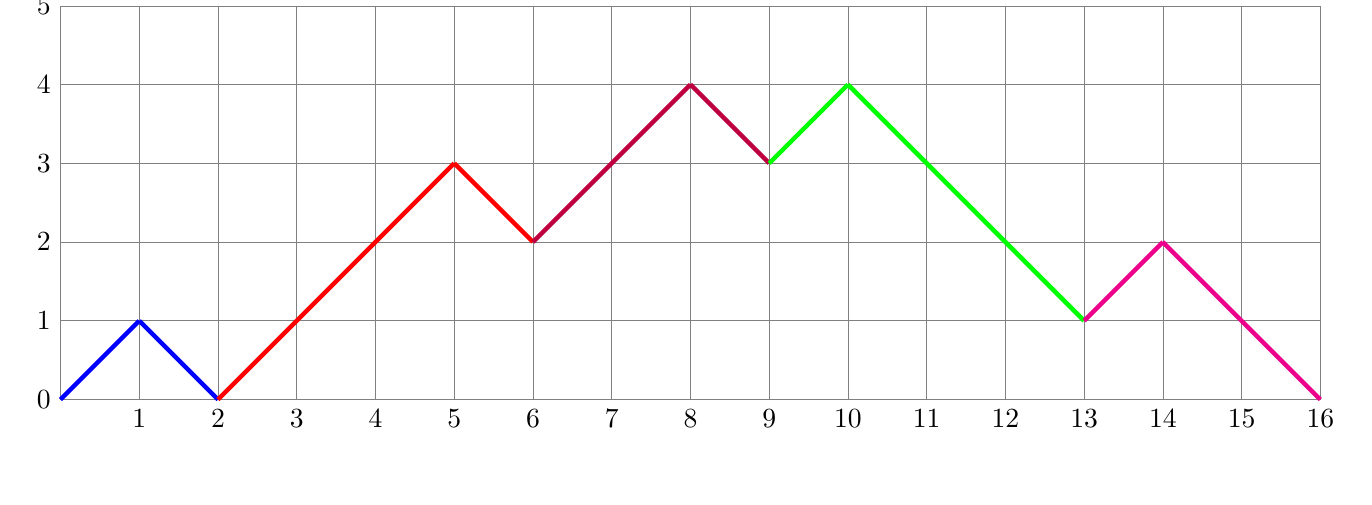
\begin{tikzpicture}[scale=1][H]
    % Draw the grid and diagonal
    \draw[help lines] (0,0) grid (16,5);

    \node[left] at (0,0) {0};
    \node[left] at (0,1) {1};
    \node[left] at (0,2) {2};
    \node[left] at (0,3) {3};
    \node[left] at (0,4) {4};
    \node[left] at (0,5) {5};
    \node[below] at (1,0) {1};
    \node[below] at (2,0) {2};
    \node[below] at (3,0) {3};
    \node[below] at (4,0) {4};
    \node[below] at (5,0) {5};
    \node[below] at (6,0) {6};
    \node[below] at (7,0) {7};
    \node[below] at (8,0) {8};
    \node[below] at (9,0) {9};
    \node[below] at (10,0) {10};
    \node[below] at (11,0) {11};
    \node[below] at (12,0) {12};
    \node[below] at (13,0) {13};
    \node[below] at (14,0) {14};
    \node[below] at (15,0) {15};
    \node[below] at (16,0) {16};
    \draw[ultra thick, blue] (0,0) -- (1,1);
    \draw[ultra thick, blue] (1,1) -- (2,0);
    \draw[ultra thick, red] (2,0) -- (5,3);
    \draw[ultra thick, red] (5,3) -- (6,2);
    \draw[ultra thick, purple] (6,2) -- (8,4);
    \draw[ultra thick, purple] (8,4) -- (9,3);
    \draw[ultra thick, green] (9,3) -- (10,4);
    \draw[ultra thick, green] (10,4) -- (13,1);
    \draw[ultra thick,  magenta] (13,1) -- (14,2);
    \draw[ultra thick,  magenta] (14,2) -- (16,0);
\end{tikzpicture}
$$

Then we reflect the Dyck path over the vertical line to get the corresponding Dyck path to the $123$-avoiding permutation $\pi$:

$$
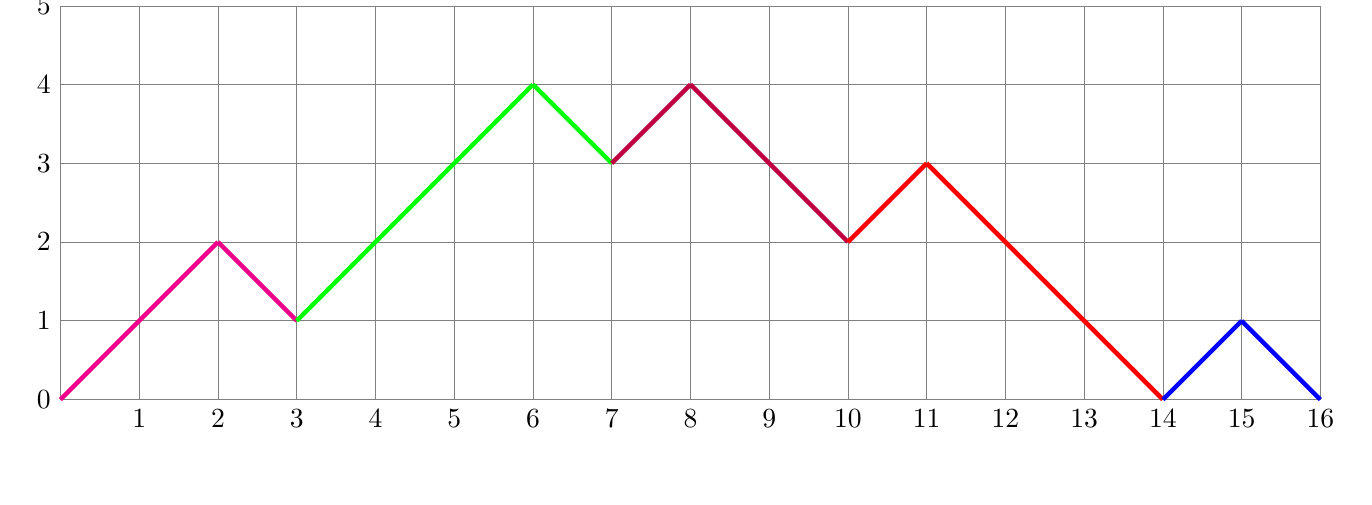
\begin{tikzpicture}[scale=1][H]
    % Draw the grid and diagonal
    \draw[help lines] (0,0) grid (16,5);

    \node[left] at (0,0) {0};
    \node[left] at (0,1) {1};
    \node[left] at (0,2) {2};
    \node[left] at (0,3) {3};
    \node[left] at (0,4) {4};
    \node[left] at (0,5) {5};
    \node[below] at (1,0) {1};
    \node[below] at (2,0) {2};
    \node[below] at (3,0) {3};
    \node[below] at (4,0) {4};
    \node[below] at (5,0) {5};
    \node[below] at (6,0) {6};
    \node[below] at (7,0) {7};
    \node[below] at (8,0) {8};
    \node[below] at (9,0) {9};
    \node[below] at (10,0) {10};
    \node[below] at (11,0) {11};
    \node[below] at (12,0) {12};
    \node[below] at (13,0) {13};
    \node[below] at (14,0) {14};
    \node[below] at (15,0) {15};
    \node[below] at (16,0) {16};
    \draw[ultra thick,  magenta] (0,0) -- (2,2);
    \draw[ultra thick,  magenta] (2,2) -- (3,1);
    \draw[ultra thick, green] (3,1) -- (6,4);
    \draw[ultra thick, green] (6,4) -- (7,3);
    \draw[ultra thick, purple] (7,3) -- (8,4);
    \draw[ultra thick, purple] (8,4) -- (10,2);
    \draw[ultra thick, red] (10,2) -- (11,3);
    \draw[ultra thick, red] (11,3) -- (14,0);
    \draw[ultra thick, blue] (14,0) -- (15,1);
    \draw[ultra thick, blue] (15,1) -- (16,0);
\end{tikzpicture}
$$
 
\subsection{Classical Patterns of Length 4}
When considering pattern avoidance for patterns of length larger than three, the problem becomes more complex. There are 24 $(4!)$ possible permutations of ${1,2,3,4}$. These 24 permutations can be sorted into three Wilf classes: $1234$, $1342$, and $1324$ patterns. 

While the number of permutations of length $n$ avoiding the patterns $1234$ and $1242$ have been solved, $1324$ pattern avoidance poses a greater mystery. 

For the pattern $1234$ (and the other patterns in this class) a formula for the number of pattern-avoiding permutations of length $n$ was discovered by Gessel and published in 1990 \cite{Gessel1990}:

$$s_n(1234) = \frac{1}{(n+1)^2(n+2)}\sum\limits_{k=0}^n\binom{2k}{k}\binom{n+1}{k+1}\binom{n+2}{k+1}$$

The number of pattern-avoiding permutations can also be expressed as a the generating function $F_{1234}(x)$ where

$$F_{1234}(x) = \sum\limits_0^\infty s_n(1234)x^n.$$

This generating function satisfies the following linear ordinary generating function \cite{Conway&Guttman2015}:

$$(9x^5-19x^4+11x^3-x^2)\left(\frac{d^3F_{1234}(x)}{dx^3}\right)+(72x^4-153x^3+90x^2-9x)\left(\frac{d^2F_{1234}(x)}{dx^2}\right)$$

$$+(126x^3-264x^2-154x-16)\left(\frac{dF_{1234}(x)}{dx}\right)+(32-72x+36x^2)F_{1234}(x)=0$$

However, the complexity of $F_{1234}(x)$ and it's corresponding ordinary differential equation makes it impractical for actually calculating the number of permutations; for this, the formula for $s_n(1234)$ is far more useful. 

For the sequence $1342$ (and it's other varieties), the formula for number of pattern-avoiding permutations was discovered by Bóna in 1997:\cite{Bona1997}

$$s_n(1342) = (-1)^{n-1}\left(\frac{7n^2-3n-2}{2}\right)+3\sum\limits_{i=0}^n(-1)^{n-i}2^{i+1}\frac{(2i-4)!}{i!(i-2)!}\binom{n-i+2}{2}$$

This can also be represented by the following ordinary generating function:

$$F_{1342}(x) = \frac{32x}{-8x^2+20x+1-(1-8x)^{3/2}}$$

While a formula and generating function have been found for pattern-avoiding permutations for both $1234$ and $1342$ patterns, we do not yet have a formula for the number of $1324$-avoiding permutations, which remains an ongoing area of research. Pattern-avoiding permutations of this kind are difficult to count since there is no simple way to break the $1324$ pattern into small parts. However, there are several researchers working on improving the upper and lower growth bounds for $s_n(1324)$ as well as calculating the number of pattern-avoiding permutations for larger values of $n$.


One aspect of $1324$-avoiding permutations undergoing research is the bounds for the growth constant. Currently, one of the best estimates for this was made using a Monte Carlo computational algorithm that place the exponential growth coefficient in the range $[10.71,11.83]$.\cite{Conway&Guttman2015} Through computational algorithms and model approximations, mathematicians are now able to calculate values of $s_n(1324)$ for lower values of $n$ and approximate for permutations of greater length. These advancements are significant. After all, in 2005, mathematician Doron Zeilberge declared "Not even God knows the number of 1324-avoiders of length 1000", and a just decade later, Conway and Guttman estimated that $s_n(1324) = 5+1 \times 10^{1017}$ (they did note that they were making no Messianic claims with this estimate).\cite{Conway&Guttman2015}



\section{Generalized Patterns}
So far, we have explored various aspects of classical pattern-avoiding permutations. However, there are various other types of pattern-avoiding permutations, such as generalized patterns.

\begin{defn}\index{generalized pattern}
A {\bf generalized pattern} is a permutation in which a dash may or may not exist between each digit. Some permutation $\pi$ is said to contain this pattern if there exists some subsequence in $\pi$ where the pattern occurs and there are no digits separating the adjacent parts of the pattern.
\end{defn}

For example, the sequence $615243$:

\begin{enumerate}
\item \underline{Contains} the pattern $41-23$ (the subsequence $6124$)

\item \underline{Avoids} the pattern $4-123$ (there exist additional digits within the increasing subsequence).

\end{enumerate}

We should also note that all classical patterns can be written as generalized patterns where dashes exists between each digit. For example, the classical pattern $132$ can be written as the generalized pattern $1-3-2$ since the pattern does not need to occur contiguously.

Generalized patterns allow us to add more restrictions to classical patterns and thus increase the number of connections between pattern-avoiding permutations and other mathematical concepts. 

\begin{prop}
    
    The number of $1-32$ avoiding permutations of length $n$, $s_n(1-32)$, is equivalent to the number of ways the sequence $\{123...n\}$ can be divided into non-empty sets. \cite{Claesson2001}
\end{prop}

\begin{proof}
Let $G_n$ be the set of the number of ways to divide the sequence $\{123...n\}$ into non-empty sets (we will call these subsets "blocks". Let $S_n(1-32)$ be the set of the permutations of length $n$ that avoid the generalized pattern $1-32$. We must prove a bijection between these two sets.

First, we must standardize the way elements of the set $G_n$ are written. We write each element so that the sequences within each block are increasing and the blocks are arranged so that the minimum value in each block is in decreasing order. Following these rules, $\{\{1\},\{2\},\{34\}\}$ (which is an element of the set $G_4$), would be written as  $\{\{34\},\{2\},\{1\}\}$.

In its standard form, we can see that if we remove the divisors, every element of the set $G_n$ avoids the pattern $1-32$. The pattern $1-32$ requires an increasing subsequence of length $2$; whic cannot occur in the same block in a standardized element of $G_n$. This increasing subsequence also cannot occur between two separate blocks since the standardization arranges blocks so that the minimum values of each block is decreasing. 

We can also see that every element of $S_n(1-32)$ can become an element of $G_n$ by inserting divisors between each decreasing sequence. Therefore, there exists a one-to-one correspondences between the sets $G_n$ and $S_n(1-32)$.


    
\end{proof}




\section{Other Interesting Properties}

\subsection{Permutation Strongly Avoiding A Pattern}

We have a permutation $\pi = \pi_1\pi_2\pi_3\ldots\pi_n$ of the set $[n]$, which means that when we apply $\pi$ to $[n]$, we transform $[n]$ to $\pi$ based on the rule below: 

\begin{centering}
   \begin{align*}
    1 &\xrightarrow{\text{swapped with number at pos. $\pi_1$ in $[n]$}} \pi_1\\
    2 &\xrightarrow{\text{swapped with number at pos. $\pi_2$ in $[n]$}} \pi_2\\
    3 &\xrightarrow{\text{swapped with number at pos. $\pi_3$ in $[n]$}} \pi_3\\
    &\ldots\\
    n &\xrightarrow{\text{swapped with number at pos. $\pi_n$ in $[n]$}} \pi_n
\end{align*} 
\end{centering}

Therefore, the square of $\pi$ ($\pi^2$) is the outcome of when we apply $\pi$ onto $\pi$ ($\pi(\pi)$) again, and we get the new permutation of $[n]$ $\pi^{'} = \pi^{'}_1\pi^{'}_2\pi^{'}_3\ldots \pi^{'}_n$:

\begin{centering}
   \begin{align*}
    \pi_1 &\xrightarrow{\text{number at pos. $\pi_1$ in $\pi$}} \pi_1^{'}\\
    \pi_2 &\xrightarrow{\text{number at pos. $\pi_2$ in $\pi$}} \pi_2^{'}\\
    \pi_3 &\xrightarrow{\text{number at pos. $\pi_3$ in $\pi$}} \pi_3^{'}\\
    &\ldots\\
    \pi_n &\xrightarrow{\text{number at pos. $\pi_n$ in $\pi$}} \pi_n^{'}
\end{align*} 
\end{centering}

\begin{defn}
    Let $\sigma$ be a permutation of the set $[m]$ where $m \leq n$ such that $\pi$ avoids $\sigma$. We can say that $\pi$ is strongly $\sigma-$avoiding\index{strongly $\sigma-$avoiding} if both $\pi$ and $\pi^2$ avoid $\sigma$.
\end{defn}

We denote the number of strongly $\sigma$-avoiding permutations of $[n]$ as $Sav_n(\sigma)$.

This number has two symmetric equivalences \cite{Bona2019}:

\begin{prop} Let $\sigma$ be a pattern, and $\sigma^{-1}$ be the inverse of $\sigma$. Then we have:

$$Sav_n(\sigma)=Sav_n(\sigma^{-1})$$
\end{prop}

\begin{prop} Let $\sigma$ be a pattern of length $m$, and $\sigma^{'}$ be the reverse complement of $\sigma$ (we reverse the order of $\sigma$, then replace each element $\sigma_i$ with $m+1-\sigma_i$). Then we have:

$$Sav_n(\sigma)=Sav_n(\sigma^{'})$$
\end{prop}

We have a special case, which is when $\sigma$ is a strictly increasing pattern ($\sigma = 1\;2\;3\;\ldots\;m$).
\begin{thm}
    For all $m \in \mathbb{N}$, if we have $n \geq (m - 1)^3 + 1$, we have $Sav_n(\sigma) = 0$ with $\sigma = 1\;2\;3\ldots m$.
\end{thm}

\begin{proof} 
Let $\pi = \pi_1\pi_2\pi_3\ldots\pi_n$ be a permutation of the set $[n]$ with $n \geq (m-1)^3 + 1$ that avoids the pattern $\sigma = 1\;2\;3\ldots m$, or an increasing subsequence of length $m$. Therefore, $\pi$ can be decomposed into $m-1$ decreasing subsequences, so the permutation's longest increasing subsequence has length at most $m-1$.

We can color these decreasing subsequences using $m-1$ colors. By the Pigeonhole Principle, every color must be used for at least $(m-1)^2$ times and at least one of the colors must be used for at least $(m-1)^2+1$ times. Let this $(m-1)^2+1$-sized decreasing sequence be $S = \pi_{i_1}\pi_{i_2}\pi_{i_3}\ldots\pi_{i_{S}}$ with $i_1 < i_2 < i_3 < \ldots < i_{|S|}$.

Now, we need to consider the positions of the elements in $\pi$ that correspond to the values in $S$. Since there are at least $(m-1)^2+1$ such positions, we apply the Pigeonhole Principle again. Among these positions, there must exist a subset of at least $m$ positions that themselves form a decreasing subsequence in $\pi$.  

Let $p_a$ and $p_b$ be two  positions where $p_a < p_b$ and the elements at these positions in $\pi$ satisfy $\pi_{p_a} > \pi_{p_b}$. When we consider the square $\pi^2$, the elements at these original positions $i_a$ and $i_b$ are determined by $\pi(\pi_{i_a})$. Because $\pi$ reverses the relative order of these $m$ elements, those same $m$ elements will necessarily form an increasing subsequence in $\pi^2$.

Therefore, if $\pi$ avoids $\sigma$, then $\pi^2$ must contain it, which means $Sav_{n}(\sigma)=0$ for $n \geq (m-1)^3 + 1$. 
\end{proof} 

\subsection{Pattern Avoidance as Generating Trees}

An interesting way to visualize pattern-avoiding permutations is through generating trees where each node represents a pattern-avoiding permutation and each level of the tree represents the length of the pattern $n$. For example, if we were to create a generating tree for the pattern $213$, we would start with our first node labeled as $1$. For the second level of the tree, each of the two branches are representative of the two possible positions where $2$ can go, either to the left or right of the $1$. At this point, our generating tree looks like this:

\begin{center}
\begin{forest}
    [1
    [21]
    [12]
    ]
\end{forest}
\end{center}

By adding on more layers, we can visualize $s_n(213)$ for larger values of $n$. With two more layers, our generating tree looks like this:

\begin{center}
\begin{forest}
for tree={s sep = .5mm}
    [1
    [21
    [321
    [4321]
    [3421]]
    [231
    [4231]
    [2431]
    [2341]]]
    [12
    [312
    [4312]
    [3412]]
    [132
    [4132]
    [1432]
    [1342]]
    [123
    [4123]
    [1423]
    [1243]
    [1234]]]]
\end{forest}
\end{center}

Note that there is no branch for $213$ since both itself and its subsequence layers would obviously contain the $213$ pattern we attempt to avoid. Since these generating trees  eliminate any pattern-contain permutation as well as it's "children" , it is an effective way to organized pattern-avoiding permutations.  This generating tree would continue infinitely since there exists some pattern-avoiding permutation of length $n$ for every possible $n$ value. A simple example of this is the sequence $\{123...n\}$, which would exists as a pattern-avoiding permutation of length $n$ in each level of the generating tree. We can also see that, as expected, the number of nodes in each layer of our tree corresponds to the Catalan numbers (since, as shown in a previous section, the number of permutations of length $n$ that avoid a classical pattern of length $3$ is equivalent to the Catalan numbers). While the above tree is a relatively simple example of a pattern-avoiding permutation, we can also visualize a more complex example, such as permutations that avoid both $123$ and $321$ patterns ($s_n(123,321)$).

\begin{center}
\begin{forest}
    [1
    [12
    [312
    [3412]
    [3142]]
    [132]]
    [21
    [231]
    [213
    [2413]
    [2143]]]
    ]
\end{forest}
\end{center}

This generating tree is a visualization of the Erdős–Szekeres Theorem, which states  that any sequence of $n^2+1$ numbers must contain a monotonic subsequence of length $n+1$. Since there are no pattern-avoiding permutations of length $5$ or more, this generating tree is finite. We can also note that this tree is symmetrical; is is expected since the two patterns being avoiding are the direct reversal of each other, and that symmetry is reflected in the tree itself.

    


\section{Applications}

\subsection{Sorting Algorithms}
In computer science, pattern avoidance has direct applications to the problem of sorting items that have some intrinsic order in a data structure. Throughout the following discussion, we consider sorting permutations of $\{1,2,\ldots,n\}$, but the results apply to any permutation of items with an intrinsic order. To be precise, for any such list of items $\{a_1,a_2,\ldots,a_n\}$, performing any of the following algorithms on that list will give the same result as if each $a_i$ were replaced with its integer index in the theoretical sorted version of the list. Thus, any such list can be thought of as a permutation of $1$ through $n$, allowing us to relate them to permutation pattern avoidance.

\subsubsection{Stack Sorting}
A stack is a data structure with two operations. We visualize the stack as a stack of dinner plates. In the first operation, an element (plate) is ``pushed'' or ``placed'' on top of the stack. In the second operation, an element is ``popped'' from the top of the stack. Stacks are often described as first-in-last-out because the first element to be pushed will always be the last element that is popped.\\

\begin{center}
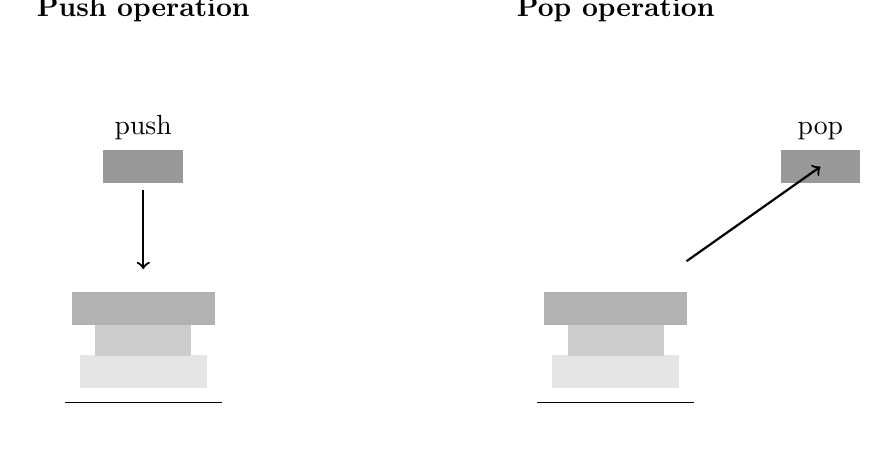
\begin{tikzpicture}[scale=1]

% left
\node at (0,5) {\textbf{Push operation}};

% stack base
\draw (-1,0) -- (1,0);

% plates (bottom to top, top one moved above arrow)
\filldraw[gray!20] (-0.8,0.2) rectangle (0.8,0.6);
\filldraw[gray!40] (-0.6,0.6) rectangle (0.6,1.0);
\filldraw[gray!60] (-0.9,1.0) rectangle (0.9,1.4);

% arrow showing push
\draw[->, thick] (0,2.7) -- (0,1.7);
\node at (0,3.5) {push};

\filldraw[gray!80] (-0.5,2.8) rectangle (0.5,3.2);


% right
\node at (6,5) {\textbf{Pop operation}};

% stack base
\draw (5,0) -- (7,0);

% plates
\filldraw[gray!20] (5.2,0.2) rectangle (6.8,0.6);
\filldraw[gray!40] (5.4,0.6) rectangle (6.6,1.0);
\filldraw[gray!60] (5.1,1.0) rectangle (6.9,1.4);

% arrow showing pop

\filldraw[gray!80] (8.1,2.8) rectangle (9.1,3.2);

\node at (8.6,3.45) {pop};

\draw[->, thick] (6.9,1.8) -- (8.6,3);

\end{tikzpicture}
\end{center}

Based on the properties of the stack, we know that, if the elements within a stack are in increasing order from top to bottom, the result of popping every element will be a sorted list. Thus, consider the following algorithm, first proposed by the seminal computer scientist Donald Knuth \cite{Bona2003}.

\begin{algorithm}[H]
\DontPrintSemicolon
    \KwIn{A list $P$ of $n$ items with ordered form $\{a_1,a_2,\ldots,a_n\}$}
    \KwOut{A new list $P'$}
    $S\leftarrow$ An empty stack\\
    \While{The size of $P'$ is less than $n$}{
        \If{$P$ is empty}{
            Pop $a_i$ from $S$ and append it to $P'$
        }
        \ElseIf{$S$ is empty}{
            Push the first element of $P$ onto $S$ and remove it from $P$
        }
        \ElseIf{The top of $S$ is greater than $P$[0]}{
            Push the first element of $P$ onto $S$ and remove it from $P$
        }
        \Else{
            Pop $a_i$ from $S$ and append it to $P'$
        }
    }
    \caption{Stack Sorting With One Stack (\texttt{stack\_sort})}
\end{algorithm}

This algorithm will be familiar to Professor Berliner's Combinatorialists. \cite{Bona2003} describes a useful alternative definition for \texttt{stack\_sort}: 

\begin{lem}
Let $P$ be a permutation of $\{1,2,\ldots,n\}$ where $n$ is in position $i$, so that $P=k_1k_2\ldots k_{i-1}nk_{i+1}\ldots k_n$. Then \begin{center}\texttt{stack\_sort}$(P)=$\texttt{stack\_sort}$(k_1k_2\ldots k_{i-1})$\texttt{stack\_sort}$(k_{i+1}\ldots k_n)n$.
\end{center}
\end{lem}
\begin{proof}
Because $n$ will only be pushed onto $S$ when $S$ is empty, everything to the left of $n$ in the permutation $P$ must pass through the stack and into $P'$ before $n$ enters $S$. Now, $n$ can only be popped from $S$ once $P$ is empty. Since stacks are first-in-last-out and $n$ was pushed before every element to its right, they must all be popped before $n$. Thus, the result of \texttt{stack\_sort} on $P$ is the result of \texttt{stack\_sort} on everything to the left of $n$, \texttt{stack\_sort} on everything to the right of $n$, and then $n$. 
\end{proof}

This leads us to pattern-avoidance. Consider that every element to the left of $n$ is part of a length-three pattern with $n$ and any element to its right. If $P$ avoids every length-three pattern which cannot be sorted by \texttt{stack\_sort}, then $P'$ will be sorted. The results of each length-three permutation are:
\begin{table}[H]
    \centering
    \begin{tabular}{ccc}
        123 $\to$ 123 & 132 $\to$ 123 & 321 $\to$ 123 \\
        213 $\to$ 123 & 231 $\to$ 213 & 312 $\to$ 123
    \end{tabular}
\end{table}

Thus, a permutation $P$ is sorted by the algorithm precisely when it avoids the pattern 231. We know that the number of such permutations of length $n$ is computed by the Catalan numbers. However, we haven't proved that the permutations that are sorted by this algorithm---permutations which avoid the pattern 231---represent every stack-sortable permutation. We will prove a similar result in the next section, but we leave the proof of this less-complicated fact to the reader as an exercise.

\begin{exc}
The operations of Algorithm 1 can be statically considered as a string of $X$s and $Y$s where $X$ represents pushing onto the stack and $Y$ represents a pop operation. For the permutation $\sigma=321$, we get the string $XXXYYY$. Prove that the number of strings which sort a permutation---and thus the number of stack-sortable permutations---is equal to the number of permutations sorted by Algorithm 1.
\end{exc} 

\subsubsection{Deque Sorting: the Kernel Method and the Schroder Numbers}
A \textit{double-ended queue} or \textit{deque} is a data structure with operations to push or pop elements from both the top and the bottom, as opposed to the one-directional nature of a stack. Counting the number of deque-sortable permutations is a hard problem, so we will start with restricting it somewhat. An \textit{input-restricted deque} (IRD) is a deque whose bottom cannot be pushed to, while an \textit{output-restricted deque} (ORD) is a deque that cannot be popped from the top. We will spend most of this section counting the number of IRD-sortable permutations.

Although we are interested in sortable permutations, it will be more effective to reframe the problem in terms of permutations that can be obtained from a given data structure. Thus, we will use the following theorem.

\begin{thm}
The number of IRD-sortable permutations of size $n$ is equal to the number of permutations of $n$ elements that can be obtained from passing a permutation through an ORD.
\end{thm}

In order to prove this through bijection, it will help to think of the different ways elements can be passed through a stack as strings of X, Y, and Z. For an ORD, Z represents popping from the bottom, while X and Y represent pushing to the top and bottom respectively. Similarly, for an IRD, Z represents pushing to the top, while X and Y represent popping from the bottom and top respectively. 

\begin{proof}
We want to show that there is a reversible mapping between an IRD-sortable permutation $\sigma$ of $n$ elements and a unique ORD string. Let $\sigma$ be such a permutation. There must be some string $s$ that sorts $\sigma$. Now, if we produce a new string $s'$ by reading $s$ in reverse, this will describe a sequence of operations that will reproduce $\sigma$ from the sorted permutation $1,2,\ldots,n$. Thus, $s'$ produces a unique permutation is obtained by passing the sorted permutation through a deque. It turns out that $\sigma$ is a member of both sets, so they are actually the same. 
\end{proof}

This result allows us to think about the problem in terms of counting unique strings that produce a valid permutation from $1,2,\ldots,n$. There are four restrictions that make a string admissible. 

\begin{defn}
A string is admissible when it satisfies the following conditions:
\begin{enumerate}
    \item There are $n$ Zs and $n$ combined Xs and Ys.
    \item Reading from left to right, the number of Zs never exceeds the combined number of Xs and Ys.
    \item Whenever the number of Zs equals the number of Xs and Ys, and there are not yet $2n$ characters, the next character is an X.
    \item The substring XZ does not occur.
\end{enumerate}
\end{defn}

Rules 1 and 2 are obvious. Rules 3 and 4 prevent two strings from producing the same permutation. When an ORD is empty, only a push to the top can occur. Because pushing an element to the top and popping from the bottom can appear subsequently in either order with the same outcome, we limit the strings to popping first and pushing second. With these restrictions, we can produce two recurrence relations for ORD strings.

Consider the number of strings with $n$ total symbols and $m$ more pushes than pops that are otherwise admissible. Denote all such strings which end in Z (a pop) with the sequence $\{h_{n,m}\}$ and all those that do not with $\{g_{n,m}\}$. Our two recurrences are $$g_{n+1,m}=2g_{n,m-1}+h_{n,m-1}$$ $$h_{n+1,m}=g_{n,m+1}+h_{n,m+1}.$$

The first recurrence comes from the fact that a sequence which does not end with a pop can have any of three operations as its second to last, with one less total element in the deque. The second recurrence comes from the fact that a sequence which does end with a pop cannot have a push to the top before it (Rule 4). Now, denote $\{b_n\}$ as the sequence which counts the number of permutations of $n$ numbers generated by an ORD. Note that $b_n$ is precisely equal to $h_{2n,0}$, the number of admissible strings of length $2n$ that leave nothing remaining in the deque. Using $g$, $h$, and a useful combinatorial trick called the kernel method, we will be able to find a closed-form generating function (but not a formula) for $b_n$.

\begin{ex}
What is the closed-form of the generating function $B(x)=\sum\limits_{n=0}^\infty b_nx^n$?
\end{ex}
\begin{proof}
Define bi-variate generating functions for our two sequences $g$ and $h$:
$$G(x,y)=\sum\limits_{n,m=0}^\infty g_{n,m}x^my^n,\ H(x,y)=\sum\limits_{n,m=0}^\infty h_{n,m}x^my^n.$$
Then, from our recurrence relation, $$\sum\limits_{\substack{n=0\\m=2}}^\infty g_{n+1,m}x^my^n = 2\sum\limits_{\substack{n=0\\m=2}}^\infty g_{n,m-1}x^my^n+\sum\limits_{\substack{n=0\\m=2}}^\infty h_{n,m-1}x^my^n,$$ which, after shifting indices and multiplying by $x$ and $y$ where appropriate, becomes $$\frac{1}{y}\sum\limits_{\substack{n,m=0}}^\infty g_{n,m}x^my^n = 2x\left(\sum\limits_{n,m=0}^\infty g_{n,m}x^my^n-\sum\limits_{n=0}^\infty g_{n,0}y^n\right)+x\left(\sum\limits_{n,m=0}^\infty h_{n,m}x^my^n-\sum\limits_{n=0}^\infty h_{n,0}y^n\right)+x.$$

The added $x$ comes from the fact that the recurrence relation only applied for $m>1$, and thus misses any terms with $x^1$. The only such term is $xy$, and it is only missing in $G(x)$ on the left. Now, if there are zero elements remaining in the deque, then an admissible string that does not end in a pop must be empty, so $g_{n,0}=0$ for all $n$ and we can eliminate it. Converting each series back into its generating function, we are left with $$\frac{G(x,y)}{y}=2xG(x,y)+x\left(H(x,y)-\sum\limits_{n=0}^\infty h_{n,0}y^n\right)+x.$$ 

The series $h(y)=\sum_{n=0}^\infty h_{n,0}y^n$ is the generating function for $h_{n,0}$, which, as stated earlier, is the function we want to determine. For now, we will move to $H(x,y)$. Applying a similar process to the recurrence relation as before, we arrive at $$\frac{H(x,y)}{y}=\frac{G(x,y)}{x}+\frac{H(x,y)-h(y)}{x}.$$ Solving for $H-h$ leads us to $$H(x,y)-h(y)=\frac{yG(x,y)-xh(y)}{x-y}.$$ We can substitute this back into our equation for $G(x,y)$, so that we get $$G(x,y)=y\left(2xG(x,y) +x\left(\frac{yG(x,y)-xh(y)}{x-y}\right)+x\right)$$ $$=2xyG(x,y)+\frac{xy^2G(x,y)}{x-y}-\frac{x^2yh(y)}{x-y}+xy.$$ Solving for $G(x,y)$, we have $$G(x,y)=\frac{\frac{-x^2yh(y)}{x-y}+xy}{1-xy-\frac{xy^2}{x-y}}=\frac{xy(x-y-xh(y)}{-2yx^2+(1-y^2)x-y},$$ which, treating $y$ as a constant, has a quadratic polynomial as the denominator.

Factoring this polynomial with the quadratic formula gives us $$r_1(y),r_2(y)=\frac{-(1+y^2)\pm\sqrt{(1+y^2)^2-4(-2y)(-y)}}{-4y},$$ so we have $$G(x,y)=\frac{xy(x-y-xh(y))}{(x+r_1(y))(x-r_2(y))}.$$ This is where the kernel method comes in. When $x=r_1(y),$ the denominator, in this case the kernel, is zero, and the function will be undefined unless the numerator is also zero. Because $r_1$ depends on $y$, the numerator must also be zero in these cases in order for $G(x,y)$ to truly be a generating function. Thus, $h(y)$ must be a function which makes the numerator zero when we substitute in $r_1$. From $$y(r_1)^2-y^2r_1-y(r_1)^2h=0$$ we get $$h(y)=\frac{yr_1(y)^2-y^2r_1(y)}{yr_1(y)^2}=1-\frac{y}{r_1(y)},$$ which is our final generating function for $h_{2n,0}=b_n$. Written out in full, as one fraction, the function is $$h(y)=\frac{3-y-\sqrt{1-6y+y^2}}{2}.$$
\end{proof}

Because this generating function does not yield a formula for $b_n$, it is difficult to see how it will be different than $C_n$, the count of stack-sortable permutations. Figure 1 plots them against the number of total permutations of $n$ numbers, so that it is easier to compare them.

\begin{figure}[htbp]
    \centering
    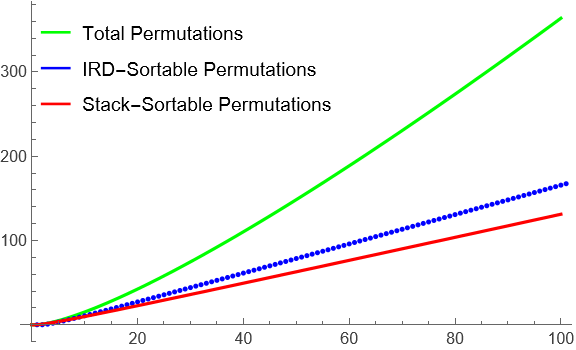
\includegraphics{media/sort_plot.png}
    \caption{On the x-axis we have $n$, and, on the y-axis, we have the number of different groups of permutations on a log scale. It is evident that the IRD improves on the stack significantly, but not in a way that inspires tremendous confidence.}
    \label{fig:example}    
\end{figure}

Expanding the power series shows us that the first few terms of $b_n$ are $1,1,2,6,22,90,394,\ldots$, which the most astute reader will recognize as the Schröder numbers. These numbers are common in combinatorics and describe many different problems, including lattice path, triangulation, and insertion of parenthesis problems. Constructing bijective proofs between these problems is a good exercise for understanding them better. In the case of pattern-avoiding permutations, The Schröder numbers count the permutations which avoid the patterns 4231 and 3241, which are also the patterns that make a permutation unsortable by an input-restricted deque. 

As for a non-restricted deque, this is still very much an open problem, and, while algorithms have been developed to solve it for specific permutations in polynomial time complexity, a generating function has yet to be discovered \cite{Bona1997}. 

\subsubsection{Stack System}
While counting IRD-sortable permutations is feasible, constructing an algorithm which correctly sorts all such permutations is not simple. Unfortunately, it is the same when many stacks are added together. \cite{knuth} showed that a sequence of $\log_2n$ stacks can sort any permutation. The $\log_2n$ number comes from the fact that each permutation can be broken into two parts: everything to the left of $n$, and everything to the right of $n$. Using $\log_2n$ stacks is enough to sort every 231 pattern. This seems promising, given that an algorithm like Algorithm 1 would theoretically have a time complexity of $O(n\log n)$, the same as many state-of-the-art sorting algorithms, but no such greedy algorithm has been found. Thus, as is the case with deque sorting, stack systems have not yet been found to be useful for sorting, although promising progress continues to be made.


\section{Conclusion}

Pattern-avoiding permutations come a wide variety of forms and thus possess a wide range of properties and applications. A relatively simple problem, such as counting the number of permutations of length $n$ that avoid the increasing pattern $123$, can become more complex and layered as connections are made to different areas of combinatorics, computer science, and other mathematical disciples. This paper explored connections such as a bijection to the Catalan numbers, stack sorting applications, and various visualizations of these pattern-avoiding permutations (Dyck paths and generating trees), yet it represents a very small portion of the associated concepts and applications. 



\printindex
%\printbibliography

\bibliographystyle{plain}
\bibliography{bibliography}

\end{document}

%Question: 